% Imported from algorithms/causal-video-vae/README.md
\chapter{因果视频 VAE 与时空压缩}\label{seedance-m01}
\moduleinfo{M01}{基础方法与机制解释}{\hyperref[src-seedance-1.0]{\texttt{seedance-1.0}}、\hyperref[src-magvit-v2]{\texttt{magvit-v2}}、\hyperref[src-wan-2.1]{\texttt{wan-2.1}}、\hyperref[src-wan21-code]{\texttt{wan21-code}}}

先从总图的表示端开始：这一章计算视频怎样进入潜空间，以及解码时怎样回到帧序列。

前面把数据看成一个向量时，暂时没有考虑向量有多大。现在换成视频，相邻帧虽然有很多重复内容，若仍把全部像素送入生成主干，计算和显存都会迅速增加。于是先引入视频 VAE：把像素映射到较小的连续潜变量，在那里学习生成，最后再解码回视频。

压缩以后便宜了，但原数据中的信息还能留下多少？这就有两个相互制约的目标。压得更小，主干更容易计算；丢掉的内容更多，细字、纹理和快速运动也更难重建。因此 VAE 既决定主干从什么规模开始计算，也限制后面能够恢复哪些细节。

\section{一段视频怎样变成潜变量}\label{seedance-m01-ux4e00ux6bb5ux89c6ux9891ux600eux6837ux53d8ux6210ux6f5cux53d8ux91cf}

用 \(B\) 表示批大小，\(F\) 表示帧数，\(H_0,W_0\) 表示原始分辨率。采用通道在前的布局，输入为：

\[
x\in\mathbb{R}^{B\times3\times F\times H_0\times W_0}.
\]

以 Seedance 1.0 的压缩配置为例，时间压缩率为 4，空间两轴各压缩 16 倍，潜变量通道数为 48。第一帧单独保留时间位置，其余帧按时间压缩，所以在 \(F=1+4k\) 时：

\[
z\in\mathbb{R}^{B\times48\times(1+k)\times H_0/16\times W_0/16}.
\]

这里的时间长度为何是首帧加压缩组数？原输入的 \(1+4k\) 帧中，首帧单独占一个位置，其余 \(4k\) 帧按四倍压缩成为 \(k\) 个位置，所以得到 \(1+k\)。空间两个方向分别除以 16，通道再变成 48。每一轴的变换都在张量里有明确位置。

编码器通常先预测后验分布的均值 \(\mu\) 和对数方差 \(\log\sigma^2\)，再通过重参数化采样：

\[
z=\mu+\sigma\odot\epsilon,\qquad \epsilon\sim\mathcal{N}(0,I).
\]

48 是采样后 \(z\) 的通道数；若实现把均值和对数方差拼在一起，该中间张量会有 96 个通道。使用后验均值还是随机采样、是否再做缩放和平移，属于模型接口的一部分，训练与推理必须保持一致。

例如，121 帧、\(480\times832\) 像素的视频会变成形状为 \codepath{B×48×31×30×52} 的潜变量。若生成主干不再切 patch，每个潜空间位置对应一个视觉 token，共有：

\[
N=31\times30\times52=48\,360.
\]

\section{为什么首帧需要单独处理}\label{seedance-m01-ux4e3aux4ec0ux4e48ux9996ux5e27ux9700ux8981ux5355ux72ecux5904ux7406}

为什么要单独保留首帧？一方面，因果编码允许它不依赖后面帧；另一方面，输入只有一张图时，时间维仍是合法的。于是图片可以看成这个视频编码过程的一个特例，同一个编码器就有机会处理两者。

\begin{figure}
\centering
\pandocbounded{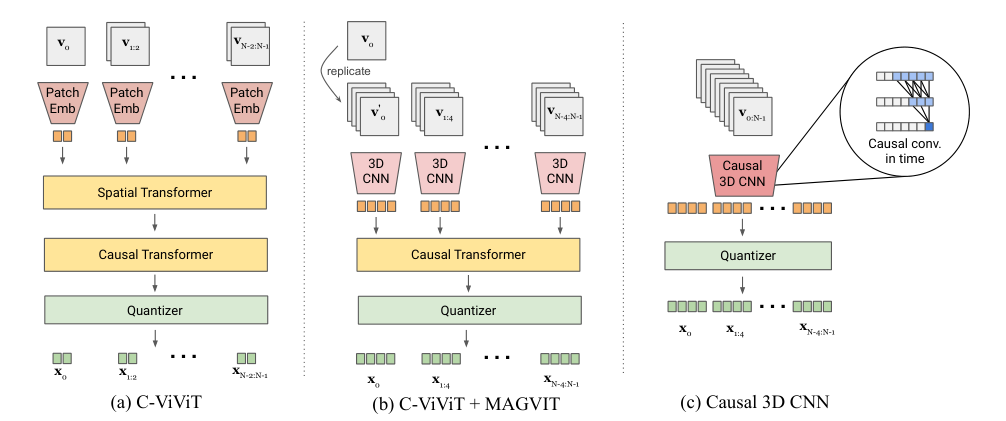
\includegraphics[keepaspectratio,alt={因果视频编码器的几种组织方式 （论文示意，来源：magvit-v2）}]{assets/seedance/figures/causal-tokenizer.png}}
\caption{因果视频编码器的几种组织方式 （论文示意，来源：magvit-v2）}
\end{figure}

图右的因果三维卷积，在时间上读取历史，在空间上仍读取邻域。这有助于理解视觉 tokenizer 怎样组织时空信息。但图中的离散量化器与这里连续 VAE 的概率潜变量不是同一种设计，借用结构示意时不能把两者直接替换。

保留首帧也意味着，有限帧数下的压缩率需要精确计算。以\textbf{元素数量}为单位，压缩后的元素与原像素元素之比是：

\[
r_F=\frac{48\left(1+(F-1)/4\right)}{3F\cdot16^2}.
\]

当 \(F\) 很大时，它趋近于 \(1/64\)；121 帧时约为 \(1/62.45\)，单张图片则是 \(1/16\)。这个比值没有考虑数据类型：原始像素可能是 uint8，潜变量可能是 BF16，不能直接把元素比当成显存字节比或视频文件压缩率。

\section{因果性来自输入索引}\label{seedance-m01-ux56e0ux679cux6027ux6765ux81eaux8f93ux5165ux7d22ux5f15}

再看“因果”在卷积里具体是什么意思。普通三维卷积的时间窗口可能覆盖前后帧；若要当前输出不读未来，就只能在时间轴左侧补齐。接着把 padding 和 stride 写进索引，才能检查这个说法是否真的成立。

设时间卷积核大小为 \(k_t\)，膨胀率为 \(\delta\)，步长为 \(s\)，左侧 padding 为：

\[
p=\delta(k_t-1).
\]

输出位置 \(j\) 读取的输入时间索引为：

\[
js-p+i\delta\le js,\qquad 0\le i<k_t.
\]

最大索引不超过 \(js\)，所以该输出没有读取未来。当核大小为 3、膨胀率为 1 时，序列 \codepath{[a,b,c,d]} 左补两个零，四个卷积窗口依次为 \codepath{[0,0,a]}、\codepath{[0,a,b]}、\codepath{[a,b,c]}、\codepath{[b,c,d]}。

PyTorch 对 \codepath{B,C,T,H,W} 张量的 padding 从最后一个维度开始填写：

\begin{verbatim}
# Conv3d 内部 padding 设为 0，空间 padding 另行计算。
x = F.pad(x, (pad_w, pad_w, pad_h, pad_h,
              dilation_t * (kernel_t - 1), 0))
y = conv(x)
\end{verbatim}

对应的时间输出长度是：

\[
F_{\mathrm{out}}=\left\lfloor\frac{F-1}{s}\right\rfloor+1.
\]

从长度式可以看到，步长设成 4，并不意味着所有输入帧数都可直接除以 4。首帧怎样处理，多出的帧怎样补或裁，最后解码怎样还原，必须是同一套约定。否则张量虽然能够接上，时间位置已经错了。

\section{整个网络怎样保持因果}\label{seedance-m01-ux6574ux4e2aux7f51ux7edcux600eux6837ux4fddux6301ux56e0ux679c}

不过，卷积这一层不读未来，是否就证明整个编码器因果了？还没有。若归一化同时统计整段时间的均值和方差，未来帧仍会改变前面的输出；跨时间注意力、重采样和特征缓存也可能带来同样的依赖。因此要沿完整计算图检查，不能停在一个卷积类上。

解码器还要处理时间展开。一个常见设计将 \(1+t\) 个潜时间位置展开为 \(1+st\) 帧；如果直接做普通 \(s\) 倍上采样，会得到 \(s+st\) 帧，需要配合首帧约定处理多出的 \(s-1\) 帧。采用 depth-to-space、插值加卷积或转置卷积时，长度和时间对齐规则各不相同，不能用统一的``裁掉尾部若干帧''替代依赖分析。

分块时问题还会再出现一次。每块若都重新补零，就相当于把每个块首当成视频起点，块边界自然可能接不上。所以除了历史特征，还得保留 stride 的采样相位：下一块从什么位置继续采样，也属于连续编码的定义。

\section{训练损失各自负责什么}\label{seedance-m01-ux8badux7ec3ux635fux5931ux5404ux81eaux8d1fux8d23ux4ec0ux4e48}

表示和长度确定后，才看这个压缩器怎样训练。一个常见写法是把重建、感知、分布约束和对抗项放在一起：

\[
\mathcal{L}=\lambda_1\lVert x-\hat{x}\rVert_1
+\lambda_p\mathcal{L}_{\mathrm{LPIPS}}
+\beta D_{\mathrm{KL}}\left(q(z\mid x)\Vert\mathcal{N}(0,I)\right)
+\lambda_a\mathcal{L}_{\mathrm{adv}}.
\]

其中 L1 看像素重建，LPIPS 看感知特征，KL 约束后验分布，判别器再提供纹理和运动监督。各项关心的量并不相同，所以权重、求和或平均的方式，以及判别器何时开始训练，都会改变优化。KL 太强可能损失细节，对抗项过早介入又可能不稳定，不能只看目标函数里有没有写齐这些名字。

最后可以反过来检查：真实视频经过编码和解码，细字、手部、快速运动与切镜还剩下多少？再扰动未来帧，看过去输出是否变化；比较整段与分块结果，看缓存是否接对。这些重建问题若还没有解决，就应先回到压缩器，而不是把丢失的细节都归因于生成主干。

\section{从极简代码到真实实现}\label{seedance-m01-ux4eceux6781ux7b80ux4ee3ux7801ux5230ux771fux5b9eux5b9eux73b0}

卷积的核心可以压缩成两步。设输入为 \codepath{B,C,T,H,W}，卷积内部不再自动补齐：

\begin{verbatim}
left = dilation_t * (kernel_t - 1)
x = F.pad(x, (pad_w, pad_w, pad_h, pad_h, left, 0))
y = conv3d(x)
\end{verbatim}

左侧 padding 决定时间依赖，空间 padding 负责尺寸。完整教学类见 \hyperref[code-causal-conv]{causal\_conv.py}；真实 VAE 的上下采样、归一化与特征缓存可直接读 \href{https://github.com/Wan-Video/Wan2.1/blob/9737cba9c1c3c4d04b33fcad41c111989865d315/wan/modules/vae.py}{Wan VAE}。
